% !TeX root = 00_Vorlage.tex
% !TeX spellcheck = de_DE
\section{Ergebnisse}
\label{sec:ergebnisse}
Im folgenden Abschnitt werden die Ergebnisse der Ausmessung des Erdmagnetfeldes, sowie die Bestimmung der Polarität eines Permanentmagneten und die Berechnung eines Stromes in einem Leiter. Alle Fehlerangaben beziehen sich auf statistische Fehler; Systematische werden gegebenenfalls separat diskutiert.

\subsection{Stärke und Inklinationswinkel des Erdmagnetfeld}
Die Messung des Erdmagnetfeldes wurde über den Magnetsensor des IOLabs gemacht und lief für etwas mehr als \( 30 \unit{s} \). Wie in \autoref{sec:Erdmagnetfeld} beschrieben, wurde das IOLab so ausgerichtet, dass eine Komponente .
In \autoref{fig:Bmean} sind die aufgezeichneten Magnetfelddaten auf die Zeit aufgetragen. Hier sieht man, dass das IOLab so ausgerichtet wurde, dass die \( B_y \) Komponente normal auf das Magnetfeld steht (und daher keinen Beitrag misst). 

\begin{figure}[H]	
	\centering
	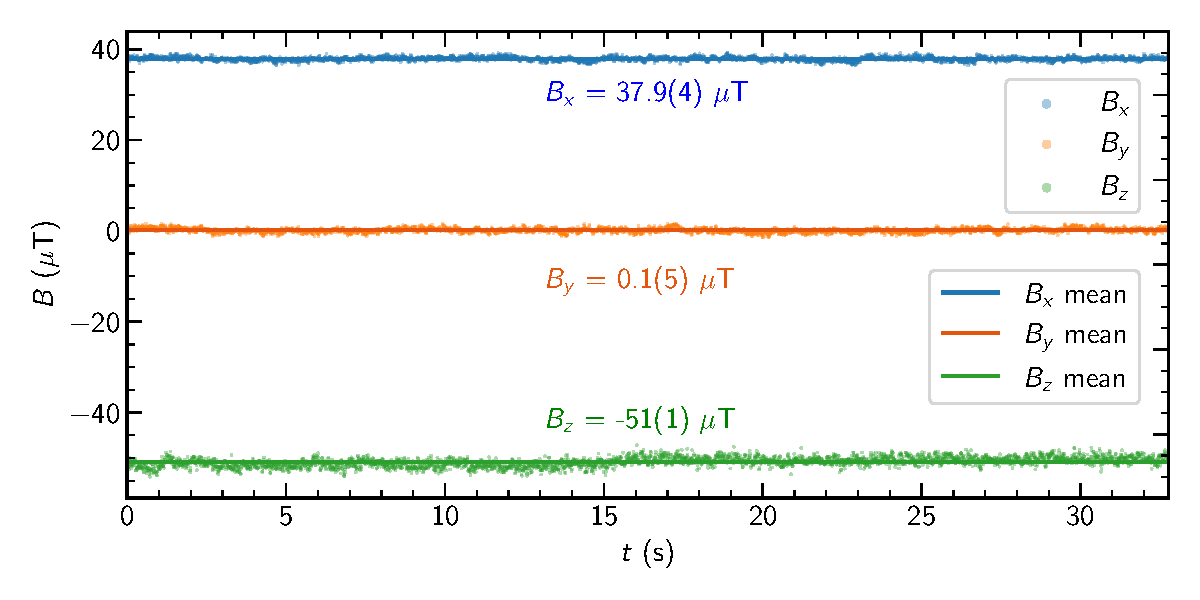
\includegraphics[width=\textwidth]{Versuch6_1}
	\caption{Das gemessene Magnetfeld in die drei kartesischen Raumrichtungen farblich unterscheidbar auf die Zeit aufgetragen. Der Mittelwert der Daten wird als durchgezogene Linie dargestellt.}
	\label{fig:Bmean}
\end{figure}

Es wurde für jede Komponente der Mittelwert gebildet und der Fehler auf die Standardabweichung gesetzt, da dann (per Definition) zwei drittel der Daten innerhalb des \( 1\sigma \) Intervalls liegen. 

Man erhält für die drei kartesischen Komponenten des Erdmagnetfeldes
\begin{equation}\label{eqn:Bxyz}
	B_x = 37.9(4) \unit{\micro T} \qquad B_y = 0.1(5) \unit{\micro T} \qquad B_z = -50.9(1.0) \unit{\micro T}
\end{equation}
. Daraus lässt sich jetzt mit \autoref{eqn:Babs} und \autoref{eqn:theta} die Stärke und Inklination des Erdmagnetfeldes berechnen und man erhält folgende Werte
\begin{equation}\label{eqn:results}
	|\vec{B}| = 63.4(9) \unit{\micro T} \hspace{3cm} \theta = \ang{53.3(6)}
\end{equation}
. Vergleicht man diese Werte mit Literaturwerten \cite{MagCal}
\begin{equation}\label{key}
	|\vec{B}| = 48.40(15) \unit{\micro T} \hspace{3cm} \theta = \ang{63.5(2)}
\end{equation}
erkennt man, dass unsere gemessenen Werte signifikant abweichen. Das liegt wahrscheinlich daran, dass am Versuchsort eine Vielzahl an metallische Objekte vorhanden waren, die Magnetfelder beeinflussen oder sogar selber erzeugen. Der Versuch wurde nämlich in einem Gebäude aus Stahlbeton durchgeführt, in einem Raum voller Elektronik und oberhalb Labore, in welchen Experimente mit elektrischen und Magnetische Felder durchgeführt werden. Es kommt daher zu systematischen Abweichungen, die verringert werden können, indem man die Messung fern von metallischen Objekten wiederholt.

\subsection{Elektromotor}
In diesem Versuch wurde 

Anhand der Stromrichtung und der Drehung kann man auf die Richtung des Magnetfeldes schließen, da auf die bewegten Ladungsträger (der Strom) die Lorentz Kraft wirkt und die Batterie zum Drehen bringt. Das Vorzeichen der Ladungsträger spielt keine Rolle, da sich dann neben dem Vorzeichen von \( q \) auch die Flussrichtung ändern würde, was sich wegkürzt. Man kann mit diesem Experiment also nicht herausfinden, welches Vorzeichen die Ladungsträger des elektrischen Stromes haben. Der Versuch wurde viermal durchgeführt und die Ergebnisse sind in \autoref{table:1} eingetragen. Die Strom- und Drehrichtung wurden beobachtet, woraus sich die Magnetfeldrichtung erschließt. Die Konfigurationen wurden dann mit \autoref{fig:Motor} verglichen und gematched. 

\begin{center}
	\captionof{table}{Stromrichtung, Drehrichtung und daraus erschlossene Magnetfeldrichtung für die vier Konfigurationen.}
	\begin{tabular}
		{@{\extracolsep{5mm}} r c c c}
		\toprule
		\makecell[t]{Konfiguration}
		&   {\makecell[t]{Stromrichtung}}
		&   {\makecell[t]{Drehrichtung}}
		&   {\makecell[t]{Magnetfeldrichtung}}\\
		\midrule
		1 & \( -\hat{x} \) & \( \circlearrowright \) & \( -\hat{z} \) \\
		2 & \( \phantom{-}\hat{x} \) & \( \circlearrowleft \) & \( -\hat{z} \) \\
		3 & \( -\hat{x} \) & \( \circlearrowleft \) & \( \phantom{-}\hat{z} \) \\
		4 & \( \phantom{-}\hat{x} \) & \( \circlearrowright \) & \( \phantom{-}\hat{z} \) \\
		\bottomrule
	\end{tabular}
	\label{table:1}
\end{center}

\subsection{Stromdurchflossener Leiter}
Ein Stromdurchflossener Leiter erzeugt ein Magnetfeld, welches im Betrag linear mit der Distanz abnimmt (Siehe \autoref{eqn:last}). Hier wird der Abstand vom Kabel zur Position des Sensors gemessen und ergibt sich mit Trigonometrischen Überlegungen und \autoref{fig:Ab2} zu
\begin{equation}\label{eqn:r}
	r = \sqrt{H^2 + (D + T)^2}
\end{equation}
, wobei \( H = 2.0(1) \unit{cm} \) und \( T = 0.9(1) \unit{cm} \) die feste Position des Hall-Effekt Sensors im IOLab sind und \( D \) die variable Distanz ist (welche Schrittweise um \( 1.0(1) \unit{cm} \) erhöht wird).

In \autoref{fig:Bcable} sind die aufgezeichneten Daten für die drei Raumkomponenten zu sehen. In x-Richtung sind (fast) keine Ausschläge zu sehen, da diese Achse parallel zum Leiter war und das Magnetfeld radial um den Leiter geht und keine parallele Komponente besitzt. In den anderen 2 Raumrichtungen sieht man 11 Ausschläge, die mit der Zeit an Magnitude abnehmen, da das IOLab ja immer weiter wegbewegt wurde und das gemessene Magnetfeld vom Leiter daher auch weniger stark war.

\begin{figure}[H]	
	\centering
	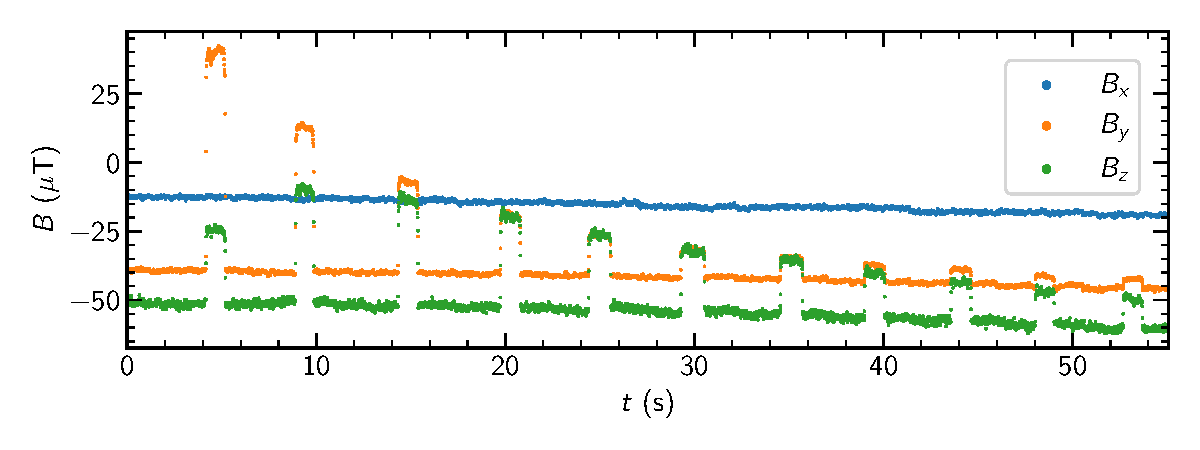
\includegraphics[width=\textwidth]{Versuch6_3}
	\caption{Das gemessene Magnetfeld in die drei kartesischen Raumrichtungen farblich unterscheidbar auf die Zeit aufgetragen. Der Mittelwert der Daten wird als durchgezogene Linie dargestellt.}
	\label{fig:Bcable}
\end{figure}

Die Analyse der Daten verlief wie folgt: Die Ausschläge wurden ermittelt und in diese wurde eine Konstante gelegt.	Von den Maxima muss noch der Untergrund abgezogen werden, um die vom Strom verursacht Änderung vom Magnetfeld zu bestimmen. Dafür wurde 2 Sekunden vor und nach dem Ausschlag die Daten gemittelt und aus diesen beiden Werten wieder der Mittelwert gebildet. Jetzt kann man die relative Änderung und daraus über die Wurzel der Quadratsummen (Siehe \autoref{eqn:Babs}) die Stärke des Magnetfeldes bestimmen. Die Fehler wurden wieder auf die Standardabweichung der Daten gesetzt.

Aus \autoref{eqn:last} erwarten uns, dass die Magnetfeldstärke proportional zum Kehrwert des Abstandes ist und aus der Konstante lässt sich dann der Strom ermitteln. In \autoref{fig:BFit} ist die Änderung der Magnetfeldes \( \Delta B \) auf den Kehrwert des Abstands \( \tilde{r} \) aufgetragen und es ist eine Gerade in rot angepasst. Die Gerade geht gezielt durch den Ursprung, da wir bei einem Abstand von \( \infty \) (und daher einem Kehrwert von 0) kein Magnetfeld spüren. Des weiteren erhöht das die Anzahl der Freiheitsgrade von 9 auf 10, was bei dem Fit nicht von großer Bedeutung ist, da die Daten nicht wirklich zum Fit passen. 

\begin{figure}[H]	
	\centering
	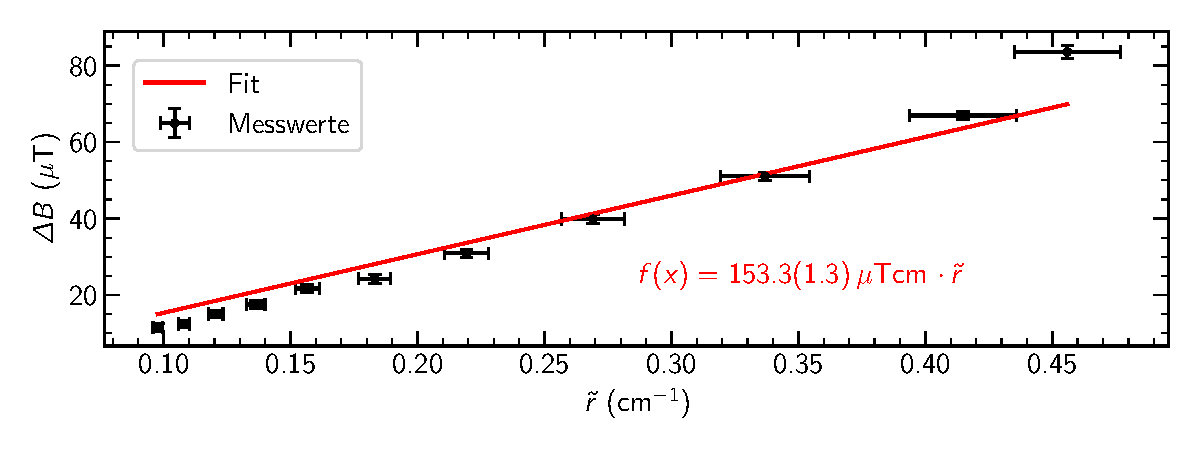
\includegraphics[width=\textwidth]{Versuch6_4}
	\caption{Die gemessene Magnetfeldänderung für verschiedene Abstände. Eine Gerade wurde in rot an die Daten angepasst.}
	\label{fig:BFit}
\end{figure}

Für die Steigung der Gerade erhält man einen Wert von \( k = 173.3(1.5) \unit{\micro\tesla\cm} \), woraus sich mit \autoref{eqn:last} ein Strom von \( I = 8.67(7) \unit{A} \) ergibt.

Nimmt man für die Batterie eine Spannung von \( U = 1.5(1) \unit{V} \) und einen Innenwiderstand von \( R_{\text{Batt}} = 0.15 \unit{\ohm} \) und für das Kabel einen Leitwiderstand von \( R_{\text{lw}} = 40.1 \unit{\ohm/km} \) an, kann man sich mithilfe des Ohmschen Gesetzes \( I = U/R \) den fließenden Strom berechnen. Setzt man hier Werte ein erhält man \( I_{\text{calc}} = 5.6(4) \unit{A} \).

Unser Wert weicht also deutlich vom theoretischen Wert ab, was an mehreren Sachen liegen kann. Einerseits entlädt sich die Batterie bei einem Kurzschluss rapide, wodurch sich die Spannung und damit der fließende Strom reduziert. Um den Strom zeitlich konstant zu halten, müsse man eine andere Spannungsquelle verwenden, die direkt am Stromnetz hängt und sich daher nicht entlädt. Zweitens wurde der Versuch in einem Gebäude voller metallischer Gegenstände durchgeführt, welche das vom Leiter erzeugt Magnetfeld verzerren. Um dieses Problem zu beheben, müsste man den Versuch an einem Ort durchführen, der möglichst Metallfrei ist. 

In der Berechnung vom Strom ist die größte Fehlerquelle die Messung des Magnetfeldes, da die Ausschläge nur sehr kurz sind und die Werte im Peak streuen. Das Problem könnte man mit einer kontinuierlichen und vor allem konstanten Stromquelle beheben, dann müsste man den Stromfluss gar nicht mehr unterbrechen, sonder könnte bei fließendem Strom den Abstand des IOLabs erhöhen.